\chapter{Fertility and Breeding Efficiency}
\label{cha:Lush_Chapter_38}
\index{Breeding efficiency|(}

The number of young produced per female per year or other unit of
time is one of the most important factors in successful animal production.
The cost of producing and maintaining the breeding females and
breeding males must be met from the sale of their products and from
the salvage value of those parents which are still alive when their breeding
usefulness is ended. As long as they are kept for breeding, beef cattle
and swine produce nothing for sale except their offspring. Dairy
cattle, sheep, goats, horses, and poultry produce milk, wool, mohair,
work, and eggs, respectively, in addition to producing their offspring.
Even in these animals a considerable part of the income --- in sheep,
more than half of it --- comes from the sale of young stock not needed for
replacements. Also, the amount of milk a dairy cow produces in her
lifetime depends much upon the frequency with which she freshens.
Unless it has a high advertising value which the breeder is in a position
to use, a phenomenally high record for one lactation may be unprofitable
if that lactation is preceded by a long dry period and if the cow is
not bred again until well along in her lactation. The production of
wool by sheep, mohair by goats, and work by horses are almost the only
returns in animal husbandry which do not depend closely upon reproductive
activity.

The number of young produced could be counted at various ages
for the purposes of measuring breeding efficiency. From the standpoint
of profits and losses it might be most logical to count the number which
reach marketing age. From the standpoint of finding the causes of high
or low breeding efficiency, more information can be had by counting
the number of young weaned or the number born alive among the
mammals or the number of birds hatched or the number of eggs laid
among poultry.

The subject of breeding efficiency receives attention in varying
degrees in different branches of animal husbandry. Ranchers pay much
attention to percentage calf crop, which is usually based on the number
of calves branded, and to lamb crop, which is usually based on the
number of lambs weaned or on the number which come back from the
summer range wherever summer and winter ranges are separated.
Poultrymen are much concerned with hatching percentages. Swine
growers often refer to the number of pigs weaned per sow and also to
the number farrowed per litter. Dairymen citing a cow's record often
add that she calved again within a certain number of months or carried
a calf a certain number of days during the lactation. Only a few dairymen
keep definite count of their percentage calf crop, as beef raisers do,
or keep track of the average length of time between calvings in their
herds. Horsemen sometimes refer to their colt crop, but the number of
mares on each farm is usually so small that each man thinks and speaks
of his colts individually. Lambert, \textit{et al.}
report\footnote{\textit{Proc. Amer. Soc. An. Prod.}, pp. 358--65, 1959}
65 live colts per year per 100 mares bred. A similar figure for Austria
is 52 colts.\footnote{Z\"uchtungskunde, 15:210.}

Variations in breeding efficiency are the net results of a complicated
interplay of genetic and environmental circumstances. Genetic causes
usually play a minor part in individual cases, being generally overshadowed
in importance by circumstances of nutrition, temporary state of
health of the dam, accident, and disease. Yet genetic causes often play a
large part in differences between the averages of groups, such as breeds
or herds.

\section*{FERTILITY}
\index{Fertility|(}

In popular usage fertility is the ability of an animal to produce large
numbers of living young. The inability to produce any offspring at all
is sterility. Either sex may be sterile, but stockmen usually speak of
sterile females as ``barren.'' Sterile is usually an absolute term meaning
that the individual is incapable, for the time at least, of producing any
young at all; but fertile is ordinarily a relative term, and high and low
fertility are used to describe differences between the numbers of young
per litter or differences in the frequencies of pregnancies.

In technical writings a distinction is sometimes made between fecundity,
fertility, and prolificacy. In that case fecundity is the potential
capacity of the female to produce functional ova, regardless of what
happens to them after they are produced; fertility is the ability to produce
living young or, in the case of poultry, to produce eggs which will
start to develop; and prolificacy is a relative term used to express
whether many or few offspring result from a given mating or from a
certain individual during its lifetime. The distinction between fecundity
and fertility is easily illustrated in poultry where a hen may have
high fecundity but her eggs may be low in fertility or hatchability; that
is, she may lay many eggs but only a few of those will start development
if incubated or perhaps only a few of those which start to develop will
go far enough to hatch into living chicks. Prolificacy is usually applied
only to females or to groups, such as breeds, strains, or herds. These
distinctions are sometimes necessary for precision in scientific writings
but are unimportant in a practical way so far as concerns the mammals.
Fertility is used here to mean in a comparative sense the ability
of parents to produce large numbers of young.

The number of functional ova released is the first limitation on fertility,
but the number actually fertilized may be much less. Failure to
be fertilized may result from several circumstances. The spermatozoa
may be few in numbers or low in vitality. Normally the male ejaculates
millions of spermatozoa at each service; therefore, the number of these
does not usually limit the number of young born. There is good evidence,
however, that in occasional instances the male is so near the
borderline of sterility that the number of normal spermatozoa is low
enough to prevent the litter from being as large as it would otherwise
be.

The spermatozoa retain their ability to fertilize the ova for only a
few hours after they are released in the female genital tract. In some
species the ova seem to be liberated at a certain stage in or just after the
heat period. If service occurs too early, the spermatozoa are dead before
the ova are liberated. If service occurs too late, the ova have passed the
period when they could have been fertilized. In dairy cattle the probability
of conception is highest when inseminations are made in the middle or later
part of the heat period. There is some evidence\footnote{Missouri Agr. Exp.
Sta., Bul. 310, p. 15.} that the number of pigs per litter in swine may be
increased by allowing two services, one early and one late in heat. Partially
offsetting this is the danger of exhausting the male by so many services that
the number or vitality of the spermatozoa in his future services to other sows
would be diminished enough to lose more than was gained by the extra service.
It is possible thus to exhaust the males, but the experimental evidence
indicates that such exhaustion rarely becomes an actual fact.

Occasionally a given mating produces no results although both individuals
later prove fertile in other matings. For example, a given mating
is made two or three times without success; then the same female is
mated to another male and conception occurs. Naturally such cases can
be interpreted in several different ways. Possibly conception would have
resulted if she had been mated at that time to the first male. The usual
number of services per conception in herds of dairy cattle, not complicated
by the presence of contagious abortion, is something like 1.8 to
2.5. With that high a percentage of unsuccessful services under what
may be regarded as average conditions, it is not surprising that there
would be occasional cases where the same service is repeated three or
more times without success and yet if repeated one more time would
result in conception.
\index{Fertility|)}

\section*{NUMBER OF YOUNG BORN}

Many of the ova which are fertilized die before they reach the stage
when they could be born normally. A few of these deaths may be the
results of lethal genes for which the embryos are homozygous and which
stop development at a certain stage. Others may be mere embryological
accidents which prevent some vital organ in the embryo from developing
as it should. A portion of those deaths may be the result of
over-crowding in the uterus, or of insufficient nutrition, particularly
with animals which have such large litters as swine and rabbits do. Part of
the evidence for this is the fact that large litters have a higher proportion
of embryos which do not complete development than small litters
do. Some embryos die from the consequences of infections in the
uterus.

Embryos which die before completing their normal development
may gradually disintegrate and be resorbed. After they are completely
resorbed, normal reproductive functioning of the female may be
resumed. Sometimes, especially if bacteria are present, some putrefaction
begins, and the embryo along with the residues of its membranes
may be aborted. If the embryo which died is one of a large litter, many
of which are still alive, as is usually the case with swine and rabbits, it
will normally be expelled along with the others when they are born. If
it died when it was extremely small, it may have had time to be resorbed
before this takes place. Even if it is not resorbed, it is often so small that
it is not noticed. If it did not die until shortly before the time of normal
birth, the breeder will merely note that there is a stillborn individual
in that litter. Many of the stillborn young in such animals as swine have
no doubt been dead for several days before birth.

\section*{VITALITY AFTER BIRTH}

The percentage of those which die between birth and marketable
age varies greatly with different kinds of animals. Much of this can be
controlled by sanitation and careful management. On farms where
swine are fairly well managed, something like two-thirds to three-fourths
of the pigs born are weaned. By far the larger proportion of
those which are not weaned are dead at birth or die within the first 48
hours after birth. Reasonably exact and useful information about the
average percentage of lambs, calves, and colts born which survive at
least to weaning time is lacking. Ranchmen often speak of a 70 per cent
calf crop, but in most regions that is more nearly a goal than an average
of what is actually achieved. Western sheepmen speak of an 80 or 90
per cent lamb crop but do not so conventionally use any one figure as
cattlemen do. The vitality of twin\index{Twins} colts is especially low as compared
with twins in other species. Uppenborn found that only 14 per cent of
the colts born as twins lived beyond the age of one year.

As the young animal grows older its mother's influence on its fate
becomes less and the effects of its own genes become relatively more
important. It is common practice in some of the sow testing work in
Sweden and Germany to use the weight of the litter at three or four
weeks of age as a measure of the sow's productivity. By putting the
weighing date as late as three or four weeks, they measure not only the
sow's fertility but also her ability to care for her pigs and produce plenty
of milk for them. Soon after three weeks of age the pigs begin to eat
other feed, and then weights are affected more and more by their own
individual abilities.

\section*{AGE AT FIRST BREEDING}
\index{Age of first breeding}
\index{Generation interval|(}

Breeding efficiency can be lowered seriously by postponing the first
breeding to a needlessly late age. Females bred at a very early age arc
apt to appear stunted, especially during the first lactation; but their
size when mature is affected very little by their having been bred early.
Extensive comparisons of early and delayed breeding with several
classes of livestock were made at the Missouri Station many years ago
and with beef cattle at the Oregon Station and with sheep at the North
Dakota Station more recently. These comparisons have shown distinct
advantages from breeding early with no disadvantages more serious
than a more stunted appearance of the early-bred females during their
first lactations. In dairy cattle, for instance, heifers bred to calve first at
less than 24 months of age produce almost as much in their first five
lactations as do heifers bred to calve first at more than 34 months. Moreover,
the early-bred heifers finish their fifth lactations at an average age
some 15 months less than. that of the late-bred heifers. Thus, almost as
much production is attained; and the feed and other maintenance costs
for over a year are saved. Breeding could be at such an early age that
difficulties at parturition would cause much trouble, but actually that
rarely happens. Troubles at parturition seem about as frequent with
older females as with younger ones.

\section*{INTERVALS BETWEEN PREGNANCIES}

Breeding efficiency of a herd or flock as a whole may be seriously
lowered by having long intervals between successive pregnancies. In
some branches of animal husbandry the breeding policy in this respect
is fixed primarily by the feed resources. An extreme example is the
range cattleman or sheepman whose feed resources may be abundant
from April to October but whose animals may have to get along on a
submaintenance ration through the winter. If he cannot have his calves
and lambs dropped before the middle of spring so that they can be
grown largely on the abundant feed of the next few months, he may
prefer to let the cows and ewes remain unbred until next year, rather
than have out-of-season calves and lambs. Moreover, ewes will normally
breed only at certain seasons of the year. For such men the problem of
keeping breeding efficiency high is concentrated in a short season of
the year and is mainly one of getting as nearly as possible 100 per cent
of the cows or ewes to conceive during that time.

For dairymen and swine producers and for beef growers in the
farming regions, there is also the possibility of increasing breeding efficiency
by rebreeding reasonably soon after calving or farrowing. Theoretically
it is possible to overdo this by breeding females so soon after
the gestation period is ended that their strength and reserve vitality can
be so exhausted that they will not produce strong offspring. Actually it
is doubtful whether such damage is often done. Natural physiological
checks and balances will guard against this danger to some extent as
they do in a state of nature. The females may fail to come in heat if
their reserves of health are low. Meanwhile each month that they are
unnecessarily kept from reproducing adds to the overhead costs of their
maintenance, which must be divided among the offspring they do produce.
There is even some possibility that each additional ovulation
adds to the scar tissue in the ovaries and thereby lowers fertility. Moreover,
each additional month brings the animal nearer the end of its
productive lifetime when one of its offspring, which might otherwise
be available for sale, must be kept to replace it.

These considerations make it likely that the wisest general policy is
to breed for the first time at an age early enough to favor the highest
lifetime production and to rebreed at almost the earliest opportunity
after each pregnancy. The data so far analyzed make it seem likely that
lifetime production by dairy cows is higher with frequent breeding and
many short lactations than it is with longer but fewer lactations. Even
when a dairyman rebreeds promptly it is difficult to keep the average
calving interval under 13 months. By raising two litters per year swine
growers who are equipped to take care of fall-farrowed pigs can reduce
very much the costs per pig of maintaining the breeding herd. In some
of the dairy regions of northwestern Europe where there is a large surplus
of skim milk, as in Denmark, some swine producers wean their pigs
at an early age and attempt to average two and one-half litters per year
per sow, although few of them actually achieve that. The average number
of litters produced per scored sow per year was 1.88 in the recognized
swine centers of Denmark for the five years ending September 1,
1934.

\begin{figure}
	\centering
    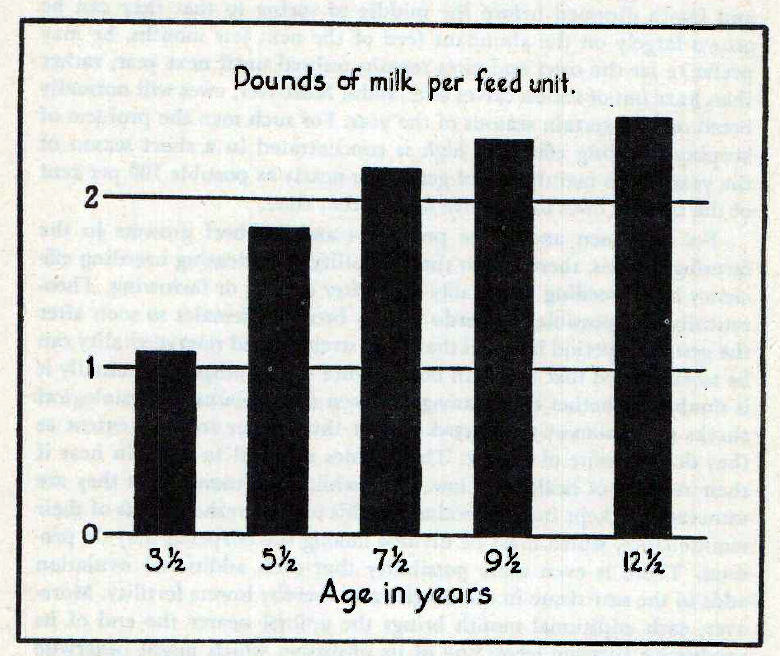
\includegraphics[width=\textwidth]{Figure_49.png}
    \caption{``It pays to have cows which last a long time.'' Chart from cow-testing
			 associations in Denmark showing how the returns in milk per unit of feed eaten by
			 a cow during her whole lifetime increase rapidly with the increasing length of her
			 productive life. (From \textit{Kvaegavlen i Jylland}, 1933.)}
    \label{fig:Lush_Figure_49}
\end{figure}
\index{Generation interval|)}

\section*{LONGEVITY}
\index{Longevity|(}

The length of life of the parent is an important part of breeding
efficiency, both from the economic standpoint and because it affects the
possibilities of improving the breed. The expenses of rearing the parent
until it is of breeding age are only partially met in most cases by the
salvage value of the parents which are still alive to be sold when they
are through producing young. Figure 49 shows a Danish analysis of cow-testing
association data. The amount of milk produced per unit of feed
eaten by the cow for her entire lifetime increases sharply as the cow's
lifetime becomes longer. The longevity of the parents has an important
effect on the possibilities of improving the breed by selection because it
affects the percentage of young which must be saved merely for replacements.
Several studies of dairy cattle indicate that under average conditions
about 20 to 30 per cent of the cows are replaced each year. This
means a productive life of four years or a little less and that something
over 60 per cent of the heifer calves born must be saved for replacements.
Seath reports an average of 3.78 calvings per cow's lifetime for
Jerseys and Holsteins in Louisiana. Barker in Canada gives 6.1 years for
the average life expectancy of dairy females and 6.0 years for registered
beef cattle. The most favorable figure yet reported from studying any
large body of data is that of Engeler, who found that the herdbook cows
of the Brown Swiss breed averaged 4.56 calves during their entire lives,
but that 69 per cent of the heifer calves born to herdbook cows were
used for breeding. Range sheep in Nevada produced 57 lambs at market
age per 100 ewes turned with the rams, but there was a complete
turnover of the ewe flock in five years. About 53 per cent of the ewe
lambs born would be needed for replacements.\footnote{Nevada Agr. Exp. Sta.,
Bul. 145.}
\index{Longevity|)}

\section*{TWINS}
\index{Twins|(}

Twins are a special case of fertility, particularly interesting in animals
where births are normally single. In some breeds of sheep there are
more twin births than single births.\footnote{\textit{Scientific
Agriculture}, 22:11--17, 1941.} In some other breeds less than
one-fifth of the births are twins. Goats are rather similar to sheep in
the frequency of twinning. Johansson summarized the records of nearly
a million births in cattle and found that l.88 per cent of all births in
``dairy breeds'' were twins. The corresponding figure for ``beef breeds''
was only 0.44 per cent. Engeler, studying 14,111 births in Brown Swiss
cattle, found that 97.3 per cent were single births, 2.7 per cent were
twins, .03 per cent were triplets, and there was one case of quadruplets.
Sanders, studying more than a million and a quarter cattle records,
found that 99.2 per cent were single births. Twins are about as rare in
horses as they are in cattle. Uppenborn found that 1.5 per cent of all
pregnancies among some 11,000 cases in horses were twins. Lauprecht,
studying the records of about 1,500 mares, each of which had foaled several
times, found that 1.5 per cent of all births were twin births. Except
for the case of identical twins\index{Identical twins}, which are common in man but rare in
the farm animals, twins are not apt to be any more alike genetically
than are full brothers and sisters born at different times. They are
usually more like each other outwardly, however, because they have
been subject to the same intrauterine environment before birth and
often are reared under much the same environment afterward.

Variations in the tendency to produce twins are inherited to some
extent. The result is that the general frequency of twinning is stronger
in some individuals and races than in others, but things other than
heredity play the major part in determining whether any particular
birth shall be a twin birth.

\section*{IDENTICAL TWINS}
\index{Identical twins}

About 50 per cent of the like-sexed twins in man are identical.
These start as a single fertilized egg but very early in their embryology
divide into two separate individuals. If this division occurs early
enough, they may even have completely separate sets of fetal membranes.
Usually they have a single chorion but separate amnions. There
are cases where the division is not complete; then the result is some
form of a double monster, ranging from almost complete separation
(the so-called ``Siamese twins'') to just a faint beginning of the doubling.
At large fairs there will often be some kind of a side-show exhibiting
living or mounted freaks of this kind from various domestic animals.

Where the separation is complete the result is two separate individuals,
of unusual genetic interest because they will be alike in all their
genes. Their coefficient of relationship will be 100 per cent, although
they may not be any more homozygous than the average of their breed
or species. Comparisons of these twins with ordinary fraternal twins
(for which the coefficient of relationship is usually 50 per cent) give us
much of our information about the importance of heredity in human
affairs. In most cases both kinds of twins are subjected to much the same
environment, yet the resemblance between identical twins is so much
greater than the resemblance between fraternal twins that there is rarely
any doubt as to whether a given pair of twins is identical if more
than three or four traits are considered. This remarkable similarity of
identical twins has been observed from ancient times. Those rare cases
where identical twins were reared apart under distinctly different environments
provide interesting evidence on the importance of heredity
and environment in man.

Identical twins are a subject of much popular interest but of little
practical importance to the breeder. They are rare in the farm animals.
Johansson estimates that $6.0 \pm 1.2$ per cent of all twin births in cattle
are identical. Bonnier's estimate is 8.5 per cent. Although they are
rare, enough have been assembled at different times and places by
Kronacher in Germany, Bonnier in Sweden, and McMeekan in New
Zealand to yield some interesting information on the interplay between
heredity and environment. Kronacher has given detailed descriptions
of many cases from cattle, including some which were double monsters,
and has emphasized their usefulness as sources of information about the
heritability of various characteristics. Identical twins seem to be much
rarer in sheep and horses if, indeed, they occur at all. There are other
animals in which they are not so rare. For instance, in the nine-banded
armadillo the normal mode of reproduction is to produce four in a
litter, the four litter mates being identical quadruplets.

\section*{TWINS WHICH ARE NOT FULL BROTHERS}

Cases are frequently reported where two individuals are born in the
same litter but are by different sires. Use is sometimes made of this in
crossbreeding experiments to furnish a more adequate control for comparing
the purebreds with the crossbreds. Boars of different breeds are
mated to a sow which belongs to the same breed as one of the boars.
Usually the resulting litter will contain some pigs by each boar. If the
breeds are so chosen that the crossbreds can be distinguished from the
purebreds by their color, this procedure provides nearly a perfect control
of environmental conditions. Somewhat more spectacular cases are
sometimes produced in animals which normally produce but one or
two young at a time. Thus, Angora does have been known to produce
twins, one of which was sired by an Angora buck while another was
sired by a Toggenburg buck. A Guernsey nurse cow at the Iowa State
College produced twins, one sired by a Hereford and the other by an
Aberdeen-Angus bull.\footnote{\textit{Journal of Heredity}, 3l:306.}
Cases are on record where a mare has produced
twins, one of which was sired by a horse while the other was sired by a
jack. Such cases are conspicuous but illustrate no new principle. Such
twins are genetically half brothers but, because of being exposed to
so nearly identical environment, are apt to resemble each other more
than ordinary half brothers do.

\section*{TWINS BORN AT DIFFERENT TIMES}

Normally in farm animals when one pregnancy has begun, the
female does not come in heat again until it is terminated. This is the
general rule, but exceptions occur. When a second pregnancy begins
before the preceding one is terminated, the usual consequence is that
the second embryo and membranes are expelled also at the time the first
pregnancy is terminated, no matter if the second embryo is still so
immature that it has no chance of living outside the mother's body.
Rarely it will happen that the second embryo is not expelled but continues
its development normally and a second birth occurs several weeks
or even months after the first one. Because such things as this are so
rare and contrary to usual experience, they are apt to be reported when
they do occur. Descriptions of such cases often appear in medical literature
as well as in stock breeding writings.
\index{Twins|)}

\section*{MANAGEMENT WHICH PROMOTES BREEDING EFFICIENCY}

Most individual variations in fertility within a breed are probably
matters of management. The principal ways to get high fertility are the
general ones of keeping the animals as free from disease as possible and
in a reasonably good nutritive condition. The probability of conception
and the number of young per conception can be noticeably increased in
sheep and swine, and probably in cattle also, by having the females in
fair condition and then distinctly improving or increasing their ration
about two or three weeks before breeding begins. This is called
\index{``Flushing''}``flushing''
and is widely practiced by sheepmen and swine growers. Range
cattlemen occasionally practice it where the price of a suitable concentrate,
such as cottonseed meal, is not prohibitive. The percentage calf
crop on the range is noticeably higher following a year when grazing
was unusually good early in the breeding season. Other specific management
to increase breeding efficiency includes breeding at a reasonably
early age, fairly prompt rebreeding, having enough males (especially
under range conditions) that they will find all females in heat and will
not have their fertility impaired by overwork, giving the males extra
feed during the breeding season, allowing only one or two services to
each female (often practical under farm conditions but not under range
conditions, of course), etc.

\index{Artificial insemination}Artificial insemination is sometimes useful
in overcoming sterility.
It is sometimes used to breed a female at a distant place to some highly
prized male without the expense of transporting one to the other. If
artificial insemination is used extensively it permits the keeping of fewer
sires and thereby effects a saving in maintenance costs. Against this
must be charged the costs of the special apparatus or skilled labor
required. By making it unnecessary to save so many sires, selection of
the sires can be more intense. That should lead to somewhat more rapid
progress although not in proportion to the number of sires which
the artificial insemination permits discarding. For example, by reference
to Table~\ref{tbl:Lush_Table_12} it will be seen that if 100 per cent represents the progress
resulting from selection among the males in one generation when
10 per cent of all males must be saved, then 117 per cent would represent
the progress expected if only 5 per cent of the males needed to be
saved, 139 per cent would represent the expected progress if only 2 per
cent of the males need to be saved and 150 per cent would represent the
progress to be expected if only 1 per cent needed to be saved. These figures
concern only that part of the progress which is made by selecting
the sires. The increasing intensity of selection among the sires would
not increase the actual merit of the offspring so rapidly, however,
because selection among the females contributes something to that, and
this selection among females would not be altered by the use of artificial
insemination. It appears, therefore, that the widespread use of artificial
insemination would increase the rates of progress somewhat but not
enough to change the prospects for breed improvement very radically.

\section*{GENETIC MEASURES TO PROMOTE BREEDING EFFICIENCY}
\index{Fertility|(}

So far as individual variations in fertility have a hereditary basis,
they are subject to selection; and the average of the herd or flock in this
respect can be changed by the same breeding methods used for changing
other characteristics. That differences in fertility are often inherited
is evident from a number of facts, such as the breed differences which
exist in sheep and swine. Breeds of cattle also differ in the percentages
of twins which they produce. Genetic literature contains many cases of
inheritance of definite malformations which result in sterility. Superficially
it seems a contradiction of terms to speak of the inheritance of
sterility, since a sterile individual would not leave offspring. Nevertheless,
sterility can be inherited just as lethal genes are; that is, carried
along in heterozygous condition. Each different gene which definitely
produces sterility must be of low frequency in the breed (just as lethal
genes are) because of the intense natural selection against it. There
might, however, be many such genes each in a different allelic series,
each individually rare and yet enough of them that all together they
would cause a noticeable amount of sterility in the whole breed. Data
collected by Pearson on the number of children per family are interpreted
by Fisher as showing that about 40 per cent of the observed variability
in human family size is genetic in origin. There is conclusive
evidence that part of the variation in longevity in Drosophila and in
man is inherited,\footnote{Consult Pearl's \textit{The Biology of Death}.}
but the direct evidence for farm animals is still
fragmentary.

There is automatically some selection for high fertility, since those
individuals with more offspring have more chances to get their sons or
daughters saved for breeding purposes. This may be canceled by the
breeder's selection for large size and excellent appearance. Individuals
born in large litters may be initially handicapped by the greater competition
and crowding. This is distinctly the case with twins in horses
and, although less extreme, is noticeable with twins in cattle, sheep, and
goats. Also, in swine the birth weights decrease and the mortality
increases as litter size increases; although size of litter is by no means the
major factor affecting birth weights and mortality, and its influence on
weaning weight is comparatively unimportant. Moreover, the sow
which has just nursed a large litter to weaning time is often thinner and
appears less attractive than one which has just weaned a few or none.
Unless careful attention is paid to their records of production, the more
productive sow is apt to be culled on account of her appearance whenever
any culling is done. All this results in some tendency to select
breeding animals which are below average in fertility themselves or
come from parents of low fertility. In a similar way some selection for
low fertility takes place in nature and may hold in equilibrium the
selection which would otherwise favor the more fertile strains. Under
many circumstances the most desirable condition with respect to fertility
is neither the maximum nor the minimum. In the very largest litters
all of the individuals are so handicapped that they cannot struggle
through to maturity as successfully as those in smaller litters. On the
other hand, those in the least fertile strains leave comparatively few
offspring when they could have reared a larger number to maturity with
almost equal success. This seems certain to cause some variation in litter
size to be epistatic so far as profitability is concerned. Studies with
swine have led to the general conclusion that a litter size of something
like 9 to 12 pigs born alive leads to the largest net profit. If the litters
are larger than this they contain too high a percentage of stillborns, and
the survivors are too small at weaning time. If the litters are smaller
than nine, incomplete use is made of the sow's ability to nurse and rear
pigs. None of the breeds of swine in the United States seem to be in danger
of exceeding this optimum as a general average for the breed, although
individual sows do exceed it frequently in single litters. Litter
size in swine has a rather low repeatability; the intraherd correlation
between the sizes of successive litters from the same sow being of the
order of one-sixth.\footnote{USDA Technical Bulletin. No. 856. 1942.} In
selecting for litter size it would be unreasonable to expect actually to
achieve each generation much more than about one-sixth of what is reached
for in the selections, especially since the boars could express their
inheritance only indirectly through the performance of their daughters.

The important practical step is to keep a reasonably complete and
up-to-date record of each female's actual production and to lay heavy
emphasis on that in all selections. By keeping the record in the form of
lifetime production, some emphasis is automatically laid on longevity.
The selection differential which can actually be made for productivity
is usually small, even when the breeder thinks he is paying much attention
to that. It is often an eye-opening experience to average the records
on that point and see just what has been accomplished. For example, in
the course of one breeding experiment at the Iowa Station (unpublished)
in which much emphasis was laid on selecting for large litters,
the data for 143 gilts farrowing in the first six years showed an average
of 7.9 pigs per litter. The 92 gilts which were saved to produce at least
one more litter averaged 8.4 pigs in their first litters. The selection
differential actually achieved at this first culling was thus only one-half
pig per litter. If the variance in litter size is about one-tenth hereditary
in the simple additive manner -- a reasonable assumption as far as the
present evidence goes -- and if selection of the boars out of prolific dams
had an equal effect, this selection would increase the average litter size
about one-twentieth of a pig per generation. With about 2\nicefrac{1}{2} years per
generation, such selection would require 50 years to increase the size of
the litter one pig! These computations are somewhat too pessimistic
since they omit the selection which takes place after the second and later
litters and the selection which takes place in saving gilts only from the
larger litters in the first place. In these same data the additional selection
differential achieved in culling sows after their second litters was
.24 pig per litter. Selection for large litters continued all through the
lives of the sows and in selecting gilts and young boars in the first place.
It is within reason to expect that the improvement in litter size might
be several times as rapid as indicated in the estimate above. The example
illustrates two things: (1) that the selection differential actually
achieved for fertility may be small even when much attention is paid to
it; and (2) that such computations may be used in setting up standards
of the average progress which may reasonably be expected.
\index{Fertility|)}

\section*{SUMMARY}

The number of young produced per female per year or other unit of
time is important in determining profits in animal husbandry. It is also
important in determining the percentage of young which must be saved
to replace their parents and in thereby setting limits on the intensity of
selection possible, especially among the females.

Fertility is limited in the first place by the number of ova produced.
It is further limited by failure of some of the ova to become implanted
or, if implanted, to develop normally enough to result in living young
at birth.

Those which die between birth and weaning cause further loss in
breeding efficiency. Much of this loss comes from faults of management,
but some is from inherent weakness of the dam and the young. As the
young grow older, their own inherent vitality and other characteristics
play a larger part in their fate, and the characteristics of their dam play
a correspondingly lesser part.

For mammals the first convenient stage for measuring differences in
fertility is when the young are born. For economic reasons or for convenience,
the number of young produced is often counted first at weaning
time.

Fraternal twins or triplets are no more like each other genetically
than ordinary full brothers and sisters. They are apt to be a little more
like each other outwardly because of having been exposed to the same
peculiarities of environment.

Identical twins, which are common in man but rare in the farm animals,
are cases where a single fertilized ovum has later developed into
two separate individuals. Such cases are unusually interesting to students
of heredity because the two twins have identical inheritance.
Their unusual likeness, as compared with that of ordinary fraternal
twins, furnishes an opportunity to estimate the relative importance of
heredity and environment.

Individuals born of the same mother at the same time may occasionally
be half brothers, having been sired by different males.

In very rare cases a second pregnancy begins before the preceding
pregnancy has terminated. Usually the younger embryo is expelled
along with the older when the older one is born. In rare cases the
younger embryo is retained and may be born several weeks or months
later.

Longevity of the parents is important in breeding efficiency both
because it spreads the cost of their rearing over a longer productive life
and because it permits more intense selection of the smaller percentage
of replacements needed.

Policies of management which promote breeding efficiency include
such things as: keeping the animals reasonably free from disease and in
good nutritive condition, flushing, breeding at a reasonably early age,
fairly prompt rebreeding, not having too many females per male, giving
the male extra feed during the breeding season, etc.

Genetic ways of promoting breeding efficiency consist of selecting
the more fertile animals, with especial emphasis on their lifetime production
of young. While it is probable that most of the ordinary individual
variations in fertility are matters of management, yet some of
these variations are hereditary, and some degree of success can be had
by selecting for them, using the same methods as are used in breeding
for other characteristics which can be manifested in one sex only. To do
such selecting it is essential that up-to-date records of lifetime productivity
be kept on each female.
\index{Breeding efficiency|)}

\section*{REFERENCES}

\begin{hangparas}{0.5in}{1}%
Briggs, Hilton M. 1936. Some effects of breeding ewe lambs. N. Oak. Agr. Exp.
Sta., Bul. 285.

Castle, W. E. 1924. The genetics of multi-nippled sheep. Jour. of Heredity, 15:75--85.

Chapman, A. B., and Casida, L. E. 1935. Factors associated with breeding efficiency
in dairy cattle. Proc. Amer. Soc. An. Prod. for 1934, pp. 57--59.

---. 1936. Length of service period in relation to productive and reproductive
efficiency in dairy cows. Proc. Amer. Soc. An. Prod. for 1935, pp. 66--70.

---, and Dickerson, G. E. 1936. The relation of age at first calving to
butterfat production in the first five lactations. Proc. Amer. Soc. An. Prod.
for 1936.

Crew, F. A. E. 1925. Animal genetics. pp. 296--311. Edinburgh: Oliver and Boyd.

Dow, G. F. 1932. Costs and returns in producing milk, raising heifers, and keeping
herd bulls in Maine. Maine Agr. Exp. Sta., Bul. 361.

Engeler, W. 1933. Die Ergebnisse statistischer Auswertung 40-jahriger Herdebuchaufzeichnungen
beim schweizerischen Braunvieh. Bern: Verbandsdruckerei A.G.

Fisher, R. A. 1930. The genetical theory of natural selection. pp. 194--99. Oxford
University Press.

Fleming, C. E., et al. 1940. Range sheep production in northeastern Nevada. Nevada
Agr. Exp. Sta., Bul. 151.

Johansson, Ivar. 1931. The sex ratio and multiple births in cattle. Zeit. f. Z\"ucht.,
Reihe B, 24:183--268.

---. 1933. Multiple births in sheep. Proc. Amer. Soc. An. Prod. for 1932,
pp. 285--91.

Kronacher, C., and Sanders, D. 1936. Neue Ergebnisse der Zwillingsforschung beim
Rind. Zeit. f. Z\"ucht. Reihe B, 34:1-172.

Lloyd-Jones, Orren, and Hays, F. A. 1918. The influence of excessive sexual activity
of male rabbits. Jour. Exp. Zool., 25:463--97.

Lovell, R., and Hill, A. Bradford. 1940. A study of the mortality rates of calves in
335 herds in England and Wales. Jour. Dairy Res., 11:225--42.

Lush, Jay L., and Lacy, M. D. 1932. The ages of breeding cattle and the possibilities
of using proven sires. Iowa Agr. Exp. Sta., Bul. 290.

Lush, Robert H. 1925. Inheritance of twinning in a herd of Holstein-Friesian cattle.
Jour. Heredity, 16:273--79.

Mumford, F. B. 1921. The effect on growth of breeding immature animals. Missouri
Agr. Exp. Sta., Res. Bul. 45.

Newman, H. H. 1933. The effects of hereditary and environmental differences upon
human personality as revealed by studies of twins. Amer. Nat., 67:193--205.

Perry, E. J. (Editor). 1945. The artificial insemination of farm animals. Rutgers
University Press.

Seath, D. M., and Neasham, E. W. 1943. A study of breeding records in dairy herds.
Louisiana Agr. Exp. Sta., Bul. 370.

Smith, A. D. B., and Robison, 0. J. 1931. The average ages of cows and bulls in
six breeds of cattle. Jour. Agr. Sci., 21:136--49.

Spielman, Arless and Jones, I. R. 1939. The reproductive efficiency of dairy cattle.
Jour. Dairy Science, 22:329--34.

Uppenborn, Wilhelm. 1933. Untersuchungen \"uber die Tr\"achtigkeitsdauer der
Stuten. Zeit. f. Z\"ucht., Reihe B, 28:1--27.

von Patow, C. 1933. Genetische Untersuchungen am Schafen. Zeit. f. Z\"ucht., Reihe
B, 26:285--321.

Withycombe, Robert; Potter, E. L.; and Edwards, F. M. 1930. Deferred breeding of
beef cows. Oregon Agr. Exp. Sta., Bul. 271.
\end{hangparas}